% Source: https://tex.stackexchange.com/a/208744/6880

\documentclass[tikz,border=5]{standalone}
\usetikzlibrary{chains}
\begin{document}
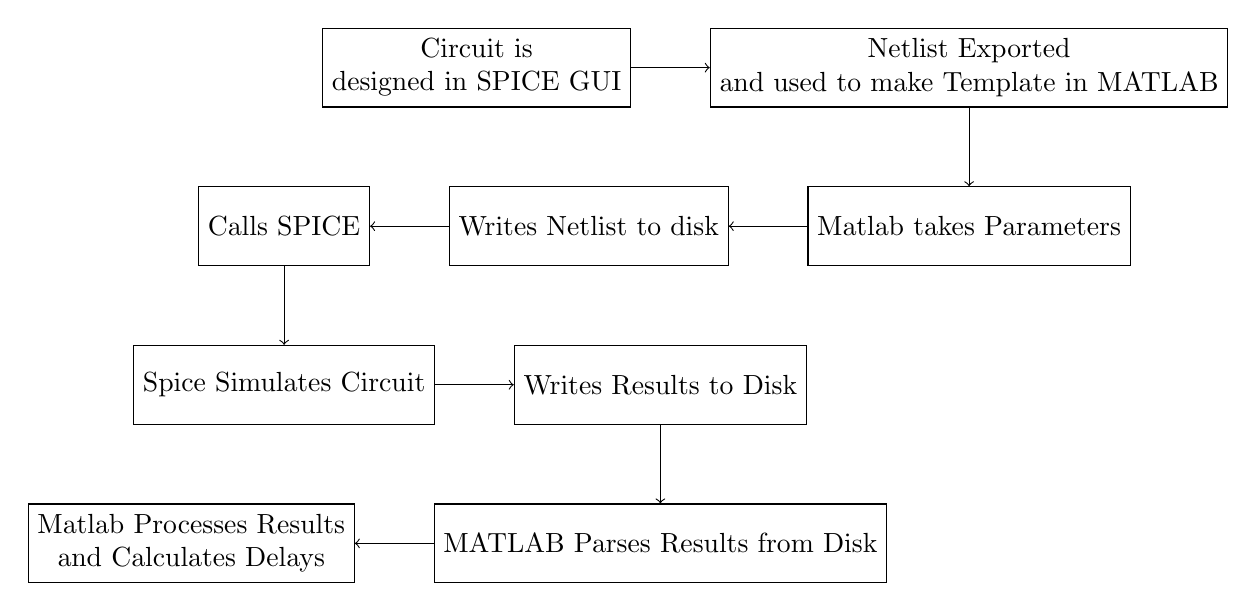
\begin{tikzpicture}
\begin{scope}[start chain=going right, every join/.style={->},
  every node/.style={draw, align=center, on chain, join, minimum height=1cm}]

\foreach \direction/\text in {%
  right / Circuit is \\ designed in SPICE GUI,
  right / Netlist Exported \\ and used to make Template in MATLAB,
  below / Matlab takes Parameters,
  left  / Writes Netlist to disk,
  left  / Calls SPICE,
  below / Spice Simulates Circuit,
  right / Writes Results to Disk,
  below / MATLAB Parses  Results from Disk,
  left  / Matlab Processes Results \\ and Calculates Delays}
    \node [continue chain/.expanded=going \direction] {\text};

\end{scope}
\end{tikzpicture}
\end{document}